\chapter{Spectrum Analyzer}
The specific target of this exploit, is the tool called the spectrum analyzer, which can be exploited through a buffer overflow.
The intended purpose of the spectrum analyzer is to identify potential problems with the connection through the cable, such as interference.
The spectrum analyzer is exposed to the local network on varying ports, though often 8080 or 6080, depending on particular cable modem.
The modem is often assigned either \mono{192.168.100.0} or \mono{192.168.100.1} as its IP address on the network. Note that this IP address is separate from the router, which often lives in the low range of \mono{192.168.0.*} or \mono{192.168.1.*}. Even if the modem is not available on the IPs above it can be discovered by running a port/ip scanner on \mono{192.168.*.*}. For instance, NMAP can be used as seen in \cref{lst:nmap_command}, which will also reveal the port of the spectrum analyzer.

\begin{lstlisting}[language=sh,firstnumber=1,label={lst:nmap_command},caption={The NMAP request to find the Spectrum Analyser},float]
    nmap 192.168.0.0/16
\end{lstlisting}

In some cases the endpoint require credentials, but so far only default credentials have been employed, granting no actual security. IPs, ports and default credentials for all tested modems have been moved from this report to the \href{https://cablehaunt.com/#faq-am-i-affected}{"Am I Affected"-FAQ} on the \exploitname{} website, to centralize the information.
A script that automatically finds and test the endpoint can be found on \href{https://github.com/Lyrebirds/cable-haunt-vulnerability-test}{GitHub}. 

\section{Overflowing the Registers}
Requests to the spectrum analyzer are sent as JSON through a WebSocket. An example of an intended request can be seen in \cref{lst:json_intended}.
\lstinputlisting[language=json,firstnumber=1,label={lst:json_intended},caption={An expected request.},float]{legit_request.json}

However, the JSON deserializer used in the spectrum analyzer, allocates a predefined amount of memory for each parameter, but will keep reading input parameters until a comma (,) is reached.
This can be exploited with a malicious request, like the one seen in \cref{lst:json_malicious}.
Here the fStartHz has a parameter value bigger than the allocated memory, and will therefore overflow and overwrite the registers.
To validate this, a researcher can attach a serial connection to the often exposed debugging ports on the modem. 
Afterwards a json package with 200 A's as the fStartHz parameter, can be sent through the WebSocket connection.
This will crash the modem and all register values will be displayed on the serial connection, showing that the program counter has changed to 0x41414141.
A more thorough walk-through of how to check this, is given in \appendixref{app:howto}.

\lstinputlisting[language=json,firstnumber=1,label={lst:json_malicious},caption={A malicious request.},float]{overflow_request.json}


\chapter{Exploiting the Buffer Overflow}
This chapter will discuss, in detail, how the MIPS architecture and eCos OS affects different exploitation strategies. It will explain how, based on calling convention and OS, \exploitname{} is most conveniently exploited using return oriented programming.

\section{Architecture and Calling convention}
The eCos OS running on the cable modem is compiled with the O32 ABI convention which has some implications on how the vulnerability can be exploited. These are the different registers and their purposes:

\begin{itemize}
    \item \textbf{\$a0 - \$a3} are registers used for parsing parameters.
    \item \textbf{\$t7 - \$t9} are caller saved register and also used as parameters if more than 4 is needed. Further are pushed to the stack.
    \item \textbf{\$v0 and \$v1} are used for return values.
    \item \textbf{\$s0 - \$s7} are callee saved registers.
    \item \textbf{\$fp} are the frame pointer but used as a s register under this calling convention.
    \item \textbf{\$sp} are the stack pointer.
    \item \textbf{\$ra} is the return address.   
\end{itemize}

There are in total eight callee saved registers, \$s0-\$s7, apart from the return address. Since the spectrum analyzer uses all eight of them, they are all, together with the return address, pushed to the stack and restored before returning. Since we can overwrite the stack during execution we have full control of program execution, via the return address, and all \$s registers. \$s registers are the most commonly used registers in normal program flow, which help when exploiting the buffer overflow.

Besides dictating how parameters are passed, the O32 ABI convention also specifics how the stack should be extended and restored. As the frame pointer is used as a normal register it is not used for referencing variables in scope of the function, instead the stack pointer is used. The stack pointer is only manipulated in the beginning and end of a function. In the beginning it will be counted down by the amount of bytes needed for the function and in the end the same value is added again. This means that the stack pointer is only being manipulated in a relative manner and never saved on the stack, excluding kernel operations such as context switch, for which exploits would be highly inconsistent if possible.

\section{Limitations}
As the stack pointer is never pushed to the stack, we cannot manipulate or read it, meaning that we cannot leak the stack pointer or use stack pivoting. This makes stack execution impractical even though it is allowed by the OS. The firmware is statically linked and there is no global offset table or procedure linkage table that can be overwritten. This leaves return oriented programing (ROP) as the best choice, since the firmware is not running with position independent execution and there is no address space layout randomization, making all addresses are known before hand. Further more, the firmware is statically linked with most of glibc available leaving us with a lot of gadgets.

\section{Return Oriented Programming}
\label{sec:return_sriented_rrogramming}
As we have program counter control and control all \$s registers, we call any existing code in the system with any context we want. Furthermore, if we skip the initial save to stack of registers, all gadgets it will restore used \$s registers and the return address from our originally overwritten stack and push stack pointer, making it ready for the next gadget. This means that we can create a fully customizable ROP chain from our originally overwritten stack.

Although we are not able to execute our own code yet, ROP enable us to execute existing code on the system in a turing-complete manner and manipulate the system extensively.
This can be used to construct a shell with external root access to the CM, allowing remote access to the system.
The specific ROP chain needed varies from modem to modem, but complete example ROP-chains can be found for \href{https://github.com/Lyrebirds/technicolor-tc7230-exploit}{Technicolor TC7230} and \href{https://github.com/Lyrebirds/sagemcom-fast-3890-exploit}{Sagemcom F@st 3890} on GitHub. A thorough explanation of a complete example can also be found in \appendixref{app:technical_replication} where an existing telnet server with root access is opened up for external access.

% \begin{figure}
%   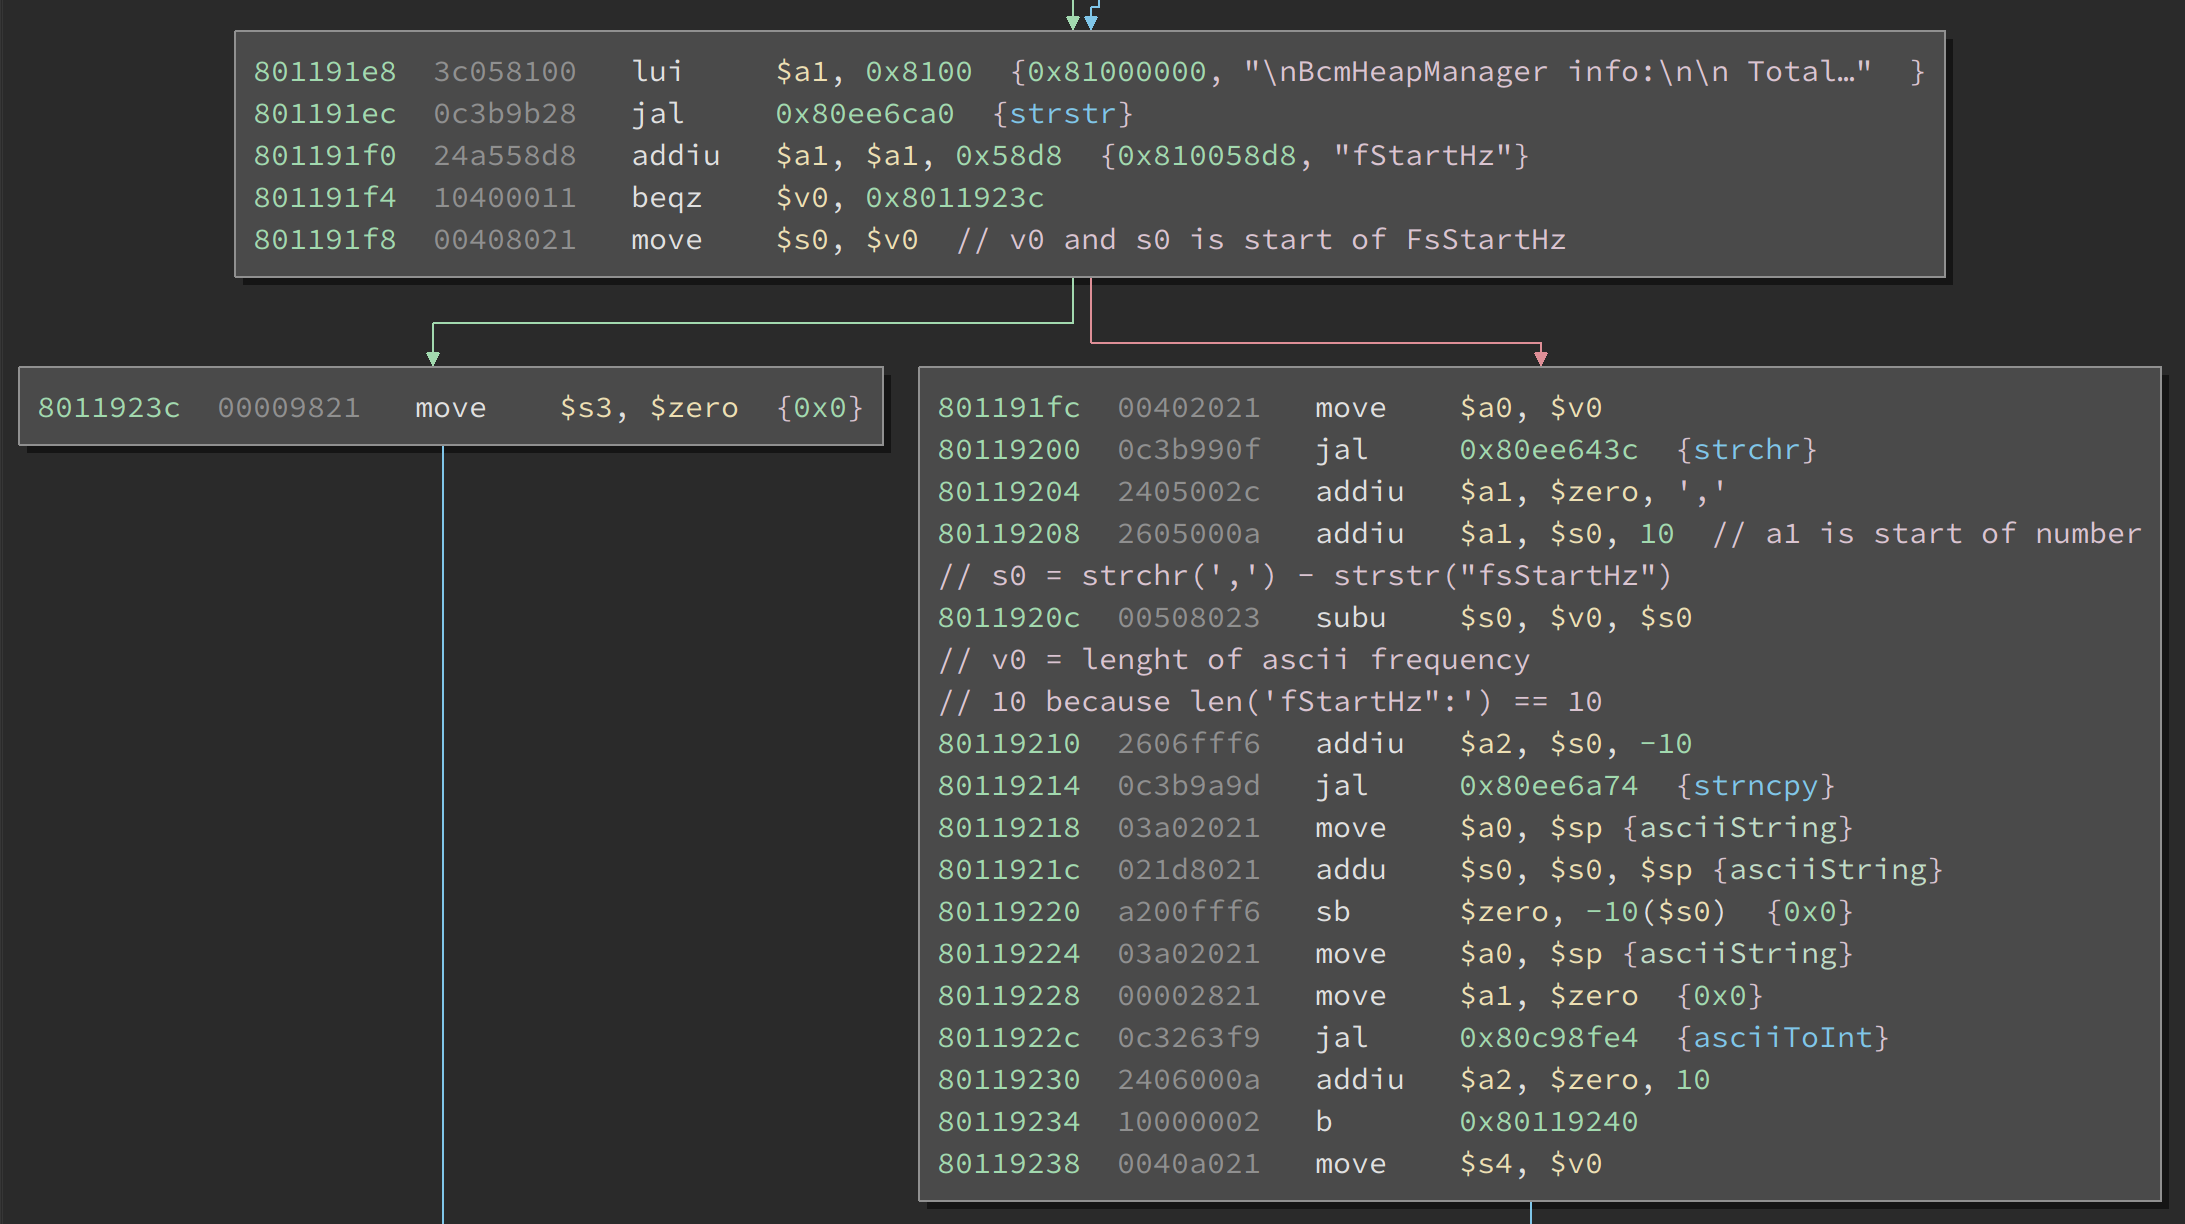
\includegraphics[width=\linewidth]{../graphics/spectrum.png}
%   \caption{Buffer overflow in beginning of stack as strncpy copies until it reaches a comma}
%   \label{fig:spectrum}
% \end{figure}
